\section{Odraz míčku}
\label{sec:odraz-micku}

Samotný odraz je pro tuto práci nejdůležitější. Tedy bude probrán velmi
podrobně. Důležitým předpokladem je, že $\speed{1}$ a $\spin{1}$ jsou hodnoty přímo
před odrazem. Díky tomuto předpokladu nemusíme uvažovat let míčku
popsaný v \myref{sekci}{sec:let-micku} ani jeho letové vlastnosti.

Problém je i tak stále velmi komplexní, protože na odraz má vliv hned několik
proměnných. Ty společně s charakteristikou celé odrazové periody budou popsány v
této sekci.

Obecně se všechny proměnné v tomto problému dají rozřadit do tří kategorií:

\begin{description}
 \item[Nezávislé] Pro tuto práci to jsou: $\speed{1}$, $\spin{1}$ a $\angle{1}$.
 \item[Závislé] Analogicky se jedná o: $\speed{2}$, $\spin{2}$ a $\angle{2}$.
 \item[Kontrolované] Jde především o materiálové konstanty:
  vertikální/horizontální koeficient restituce ($e_{x/y}$), koeficient smýkavého
 tření ($\mu$), poloměr ($R$), koeficient momentu hybnosti ($\alpha$),
 vzdálenost geometrického středu od působení normálové síly ($D$).
\end{description}

Závislé a nezávislé proměnné jsou znázorněné na \myref{obrázku}{fig:odraz-micku}.
Nezávislé jsou proměnné před odrazem a na nich závisí proměnné po odraze.
Kontrolované proměnné na \myref{obrázku}{fig:odraz-micku} nejsou, ale stále je
důležité je uvést pro replikovatelnost výsledků. Také budou z pravidla přebírány
z odborné literatury, a tedy nebudou v této práci měřené.

\begin{figure}[htbp]
 \centering
 \documentclass{article}
\usepackage{tikz}
\usepackage{xcolor}
\usepackage{mathtools}

\definecolor{darkgreen}{rgb}{0.0,0.5,0.0}
\begin{document}

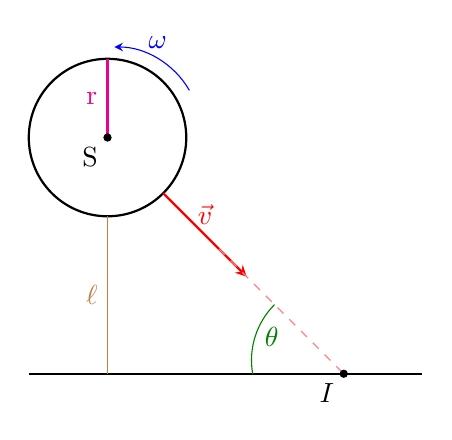
\begin{tikzpicture}
	%ball
	\draw[thick] (0,0) circle (1);
	%radius
	\draw[magenta,thick] (0,0) --node[midway,left] {r}++ (0,1);
	\node[fill=black,circle,inner sep=0pt, minimum size=3pt](s) at (0,0) {};
	%center
	\node[below left](slabel) {S};

	%speed
	\draw[red,thick,-stealth](-45:1) --node[above] {$\vec{v}$}++ (-45:1.5);
	\draw[red!50,dashed](-45:2) -- (-45:4.3);

	%graund
	\draw[thick] (-1,-3) -- (4,-3);

	%vercial length
	\draw[brown] (0,-1) --node[left] {$\ell$}++ (0,-2);

	%angle
	\node[fill=black,circle,inner sep=0pt, minimum size=3pt](naraz) at (3,-3)
	{};
	\node[below left] at (naraz) {$I$};

	\draw[darkgreen] (-45:3) arc[
			start angle = 135,
			end angle = 190,
			radius = 1,
		] node[midway,right] {$\theta$};

	%angular velocity
	\draw[blue,-stealth] (30:1.2) arc(30:90:1.1) node[midway,above] {$\omega$};
\end{tikzpicture}
\end{document}



 \caption{Síly a veličiny působící na míček při odrazu}
 \label{fig:odraz-micku}
\end{figure}

\subsection{Koeficienty restituce}
\label{ssec:koeficienty-restituce}
Koeficient restituce ($e$) vyjadřuje jak moc je odraz elastický, kolik energie
se v něm ztratí. Perfektně elastický odraz s $e=1$ tedy znamená, že při odrazu
nedojde k disipaci žádné energie. Taková odraz je ovšem v praktických podmínkách
nereálný. Hodnoty $e$ jsou v rozmezí $0 \leq e \geq 1$ kde $e=0$ znamená ztrátu
veškeré energie a už nedochází k žádnému odrazu.
\autocite{ahmadImpactModelsCoefficient2016,CoefficientRestitutionFormula}

Pro náš případ bude důležité rozdělit koeficient restituce na tečný a
vertikální ($e_{x/y}$). Tečnou komponentu budeme uvažovat v bodě, nebo ploše,
kde míček přichází do kontaktu s odrazovou plochou.

Jak bude popsáno v
\myref{podsekci}{ssec:treni-po-dobu-odrazu} na míček v průběhu kontaktu působí
tření, které není po celou dobu ve stejném směru. Pro tento případ by byl
nejpřesnější koeficient restituce odvozený z práce, kterou míček a odrazová
plocha vykonají za dobu odrazu. Pro jednoduchost bude $e$ zaveden podle Newtona
následovně\autocite{ahmadImpactModelsCoefficient2016}:
$e =  \sped{1}/\sped{2}$.

Rozdělení $e$ na jeho vertikální a tečnou komponentu můžeme vidět na
rovnicích \ref{eq:COR} a \ref{eq:CORR}. Na rozdíl od $e_y$ není definice $e_x$ intuitivní. Aby
byla tato definice logicky motivovaná je třeba vrátit se k obecné defnici z
předchozího odstavce.

\begin{align} 
 \label{eq:COR}
  e_y &= \frac{\sped{y2}}{\sped{y1}} \\
  \label{eq:CORR}
 e_x &= -\frac{(\sped{x2}-R\spn{\omega_2})}{{(\sped{x1}}-R\spn{1})}
\end{align}

\subsubsection{Lineární a úhlová rychlost}
\label{ssec:linearni-a-uhlova-rychlost}

Obecně by koeficient restituce měl být poměr lineární rychlosti před a po
odrazu. V našem případě musíme vzít v potaz, že míček má úhlovou rychlost, která
se s tou lineární sčítá.\autocite{WhyPeopleEdge2017,TangentialVelocityFormula}
Proto ji musíme odečíst abychom získali jen lineární složku rychlosti.

\begin{figure}[htbp]
 \centering
 \begin{tikzpicture}
 %circle
 \draw[thick] (-1,0) arc[
  start angle=180,
  end angle=360,
  radius=1
  ];
%vertical
 \draw[velcol, -stealth] (0,-1) --node[left] {$\speed{y}$} (0,-2);
%horizontal plus tangential
 \draw[velcol,-stealth] (0,-1) --node[below]
  {$\speed{x}\textcolor{black}{+}\speed{t}$} (1.5,-1);

 %only tangential
 \draw[velcol,-stealth] (0.75,-0.7) --node[right]
  {$\speed{t}\textcolor{black}{=R}\spin{}$}
  (1.3,0);

 








\end{tikzpicture}


 \caption{Tečná, horizontální a vertikální komponenta rychlosti}
 \label{fig:tecna-rychlost}
\end{figure}

Jak můžeme vidět na \myref{obrázku}{fig:tecna-rychlost}, tečná a horizontální
složka míří stejným směrem,\footnote{Rovnoběžné jsou tyto složky jen pro póly
míčku, ale mají stejné znaménko, pro všechny body na obvodu (pro $\sped{x} > 0$ a $ \spn{}
<0$). My koeficient restituce počítáme pro bod v kontaktu s odrazovou plochou
tedy zmíněné výpočty
platí.\autocite{crossBounceSpinningBall2005,hierrezueloSlidingRollingPhysics1995} Jinak by bylo zapotřebí započítat odchylku
$\speed{x}$ a $\speed{t}$.} tedy horizontální získáme jako
$\sped{x}-R\spn{}$. Tento výraz můžeme vidět
v \myref{rovnici}{eq:CORR}.

\subsection{Moment hybnosti}
\label{ssec:moment-hybnosti}
Moment hybnosti je rotační ekvivalent hybnosti a udává se k nějaké ose. V našem
případě tato osa prochází středem míčku a v \myref{obrázku}{fig:diagram} si ji
můžeme představit jako kolmou na celý obrázek. Úhlová rychlost také je udávána k
této ose.

Moment hybnosti definujme jako:
\[
 \vec{L}=I\spin{}
\]
Kde pro nás případ se moment setrvačnosti ($I$) rovná $\alpha m R^2$. 


\subsection{Tření po dobu odrazu}
\label{ssec:treni-po-dobu-odrazu}
otáčí se podle toho jestli převládá spin nebo speed ($\mu$)

\subsection{Triviální případy}
\label{ssec:trivialni-pripady}



